\section{\SecAdvanceBulkjob} \label{sec:bulkjob}
%====================================================================================

\scalerm には「一括実行機能」、いわゆるバルクジョブ機能が備わっている。
バルクジョブ機能とは、複数の独立した実験を1つのジョブとして実行する機能である。
これは、パラメタスイープ実験、初期値アンサンブル実験、
タイムスライス気候実験など、似たような設定を大量に行う場合に
便利な機能である。

バルクジョブ機能は、モデル本体(\verb|scale-rm|)の実行はもちろん、
地形・土地利用データ作成(地形コピー(第\ref{subsec:nest_topo}節)を利用しない場合に限る) (\verb|scale-rm_pp|)、初期値/境界値作成(\verb|scale-rm_init|)の他、ネスティング実験にも適用可能である。
%そして後処理ツールのnet2g(netcdf2grads\_bulkを使用)

以下の説明では、1のバルクジョブに含まれる独立した実行命令を「サブジョブ」と呼ぶこととする。
ここでは、3つの2段オンライン・ネスティング実験を例に説明する
(積分期間、もしくは計算領域中心が異なっている3つのサブジョブを想定している)。
%
各サブジョブの設定内容のうち、\verb|launch.conf|で指定される設定
(\verb|launch.conf|の\namelist{PARAM_LAUNCHER}の\nmitem{NUM_DOMAIN, PRC_DOMAINS, CONF_FILES};
第\ref{subsubsec:launch}節参照) は共通していなければならないが、
それ以外の設定内容(例えば、積分時間や使用するスキーム、1つのMPIプロセスあたりの格子数など)は
異なっていても構わない。


\begin{figure}[t]
\begin{center}
  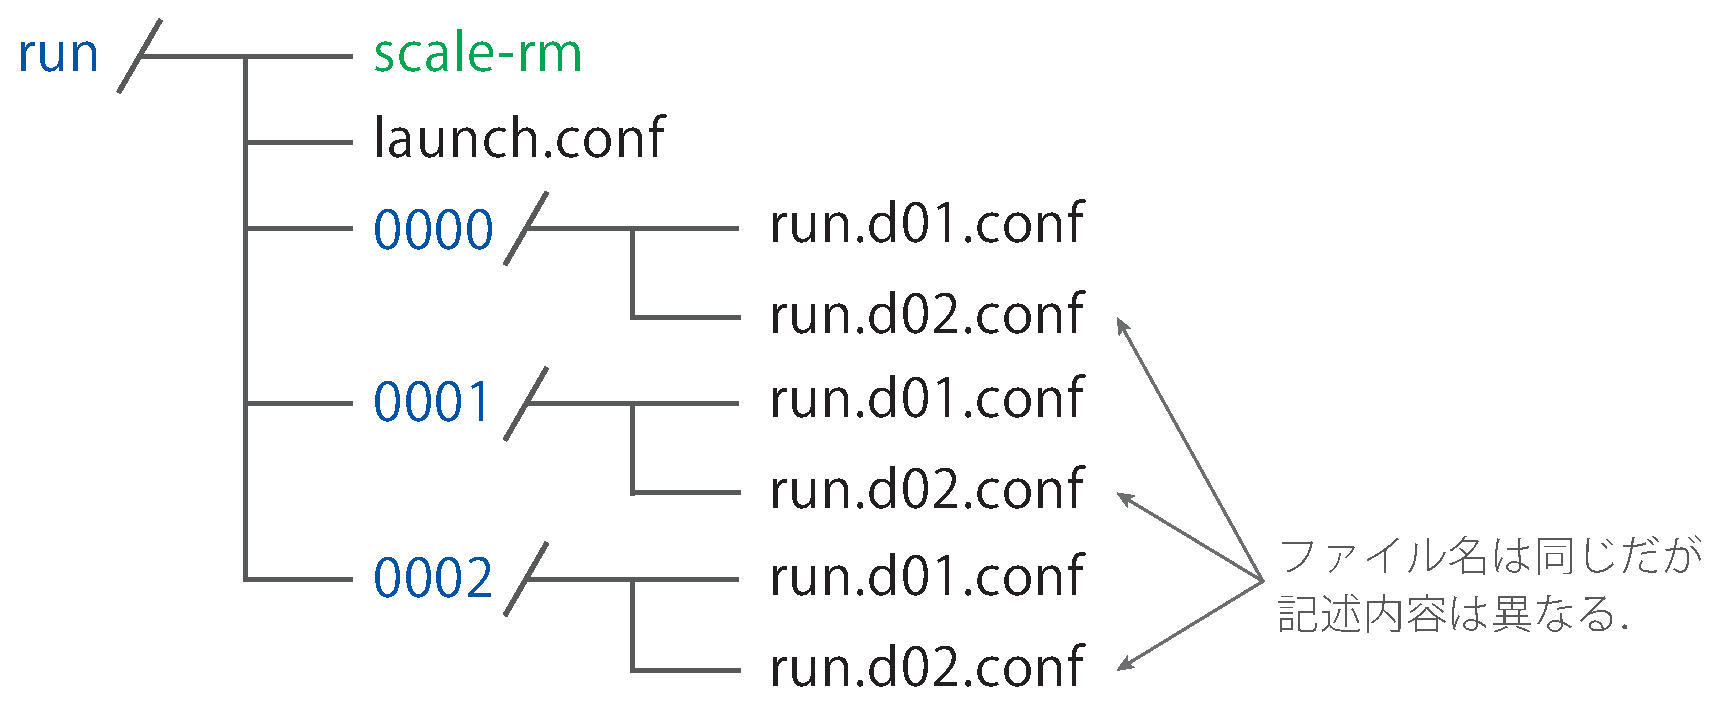
\includegraphics[width=0.6\hsize]{./figure/bulkjob_directory_structure.eps}\\
  \caption{バルクジョブ機能を使って\texttt{scale-rm}を実行する場合のディレクトリ構造. ``0000''や``0001''はジョブ番号に対応する名前のディレクトリ(ジョブディレクトリ)である。各ジョブディレクトリの中には、サブジョブの実行に必要なすべてのファイルを用意する。}
  \label{fig_bulkjob}
\end{center}
\end{figure}


バルクジョブ機能は、オンライン・ネスティングで利用した
MPIプロセスを分割・分配する機能を拡張したものである。
従って、ジョブの起動のために\verb|launch.conf|ファイルが必要になる。
オンライン・ネスティング実験とバルクジョブ機能を併用して実行する場合も
\verb|launch.conf|ファイルは1つで良い。\\

\noindent {\small {\gt
\ovalbox{
\begin{tabularx}{150mm}{lX}
\verb|&PARAM_LAUNCHER|       & \\
\verb| NUM_BULKJOB = 3,|     & サブジョブの数\\
\verb| NUM_DOMAIN  = 2,|     & ネスティング領域の数\\
\verb| PRC_DOMAINS = 9, 36,|  & \\
\verb| CONF_FILES  = run.d01.conf, run.d02.conf,| & \\
\verb|/| \\
\end{tabularx}
}}}\\

\noindent 上記は、オンライン・ネスティング実験とバルクジョブ機能を併用して実行する場合の
\verb|launch.conf|ファイルの例である。
サブジョブで設定しているオンライン・ネスティング実験の用の\verb|launch.conf|ファイルに、
\nmitem{NUM_BULKJOB}の項目を加えればよい。
それ以外の設定の詳細は、第\ref{subsubsec:launch}節の通りである。
シングルドメイン実験(ネスティングを使用しない)の場合は、
\nmitem{NUM_DOMAIN = 1}と指定し、\nmitem{CONF_FILES}に設定ファイルを1つ指定すればよい。


次に、バルクジョブの実行にあたり、まず、サブジョブの数だけ
ディレクトリ(ジョブディレクトリと呼ぶ)を用意する
(図\ref{fig_bulkjob}の\verb|0000/  0001/  0002/|)。
ディレクトリ名は、サブジョブのジョブ番号を4桁の数字で表したもので、
ジョブ番号はゼロから設定される。
それぞれのジョブディレクトリには、各サブジョブの実験に必要なすべてのファイル
(設定ファイル、入力ファイル、出力ファイルを格納するディレクトリなど) を用意する。
%
各ジョブディレクトリ内の設定ファイルは、通常の設定と同じであるが、
適切な入力ファイルが設定されているかどうか、注意が必要である。
以下にジョブ0000番のrun.d01.confの抜粋を示す。\\



\noindent {\small {\gt
\ovalbox{
\begin{tabularx}{150mm}{l}
\verb|&PARAM_IO| \\
\verb| IO_LOG_BASENAME = "0000/LOG_d01",| \\
\verb|/| \\
 \\
\verb|&PARAM_RESTART| \\
\verb| RESTART_OUTPUT       = .true.,| \\
\verb| RESTART_OUT_BASENAME = "0000/restart_d01",| \\
\verb| RESTART_IN_BASENAME  = "../init/0000/init_d01_00013046400.000",| \\
\verb|/| \\
 \\
\verb|&PARAM_TOPO| \\
\verb| TOPO_IN_BASENAME = "../pp/0000/topo_d01",| \\
\verb|/| \\
 \\
\verb|&PARAM_LANDUSE| \\
\verb| LANDUSE_IN_BASENAME = "../pp/0000/landuse_d01",| \\
\verb|/| \\
 \\
\verb|&PARAM_ATMOS_BOUNDARY| \\
\verb|     〜 中略 〜|\\
\verb| ATMOS_BOUNDARY_IN_BASENAME    = "../init/0000/boundary_d01",| \\
\verb|     〜 以下略 〜|\\
\verb|/| \\
 \\
\verb|&PARAM_HISTORY| \\
\verb| HISTORY_DEFAULT_BASENAME  = "0000/history_d01",| \\
\verb|     〜 以下略 〜|\\
\verb|/| \\
\end{tabularx}
}}}\\

\noindent 図\ref{fig_bulkjob}のとおり、
ジョブディレクトリは実行バイナリと同じ階層にある。
つまり、設定ファイルは各ジョブディレクトリの下にあるが、
入力ファイルや出力先のディレクトリは、実行バイナリの位置から見た相対パスを記述する必要がある。
従って、ジョブ0000番の実験は、実行バイナリからみてデータを出力するべきディレクトリは、
\verb|0000/|であり、出力ファイル名は\verb|0000/***|となる。
{\color{red}{例えばジョブディレクトリを付けるのを忘れて\verb|history_d01|とするなど、すべてのサブジョブで同じファイル名を設定してしまうと、同じファイルにすべてのサブジョブが書き込みを行うため、データが消失してしまうことに注意すること。}}


バルクジョブの実行は、全サブジョブを実行するのに必要なMPIプロセス数を指定し、
\begin{verbatim}
 $ mpirun  -n  135  ./scale-rm  launch.conf
\end{verbatim}
と行う。例では、一つのサブジョブあたり、$9 + 36 = 45$プロセス使用し、全体で3つのジョブを実行するので、
総計で135プロセスを必要とする。
%
実行すると得られるLOGファイルに、MPIプロセスを分割した時の情報が示されている。
LOGファイルを開くと、最初の「SCALEロゴ」のあとに下記のようなメッセージが出力される。
下記、ドメイン1のプロセス0からの出力例である。\\

\noindent {\small {\gt
\ovalbox{
\begin{tabularx}{150mm}{lX}
\verb| ++++++ Start MPI|  & \\
\verb| *** UNIVERSAL_COMM_WORLD        :        0| &; 実行環境によって値が異なる\\
\verb| *** total process [UNIVERSAL]   :      135| &\\
\verb| *** my process ID [UNIVERSAL]   :       36| &\\
\verb| *** master rank?  [UNIVERSAL]   :        F| &\\
\verb| *** GLOBAL_COMM_WORLD           :        3| &; 実行環境によって値が異なる \\
\verb| *** total process [GLOBAL]      :       45| &\\
\verb| *** my process ID [GLOBAL]      :       36| &\\
\verb| *** master rank?  [GLOBAL]      :        F| &\\
\verb| *** LOCAL_COMM_WORLD            :        4| &; 実行環境によって値が異なる \\
\verb| *** total process [LOCAL]       :        9| &\\
\verb| *** my process ID [LOCAL]       :        0| &\\
\verb| *** master rank?  [LOCAL]       :        T| &\\
\verb| *** ABORT_COMM_WORLD            :        0| &\\
\verb| *** master rank ID [each world] :        0| &\\
&\\
\end{tabularx}
}}}\\



これらのうち、\verb|[LOCAL]|と表記されている項目はドメイン内のプロセスグループ、\verb|[GLOBAL]|と表記されている項目は
ネスティンググループ、\verb|[UNIVERSAL]|と表記されて項目はジョブグループに関する情報である。
\verb|LOCAL|グループは\verb|GLOBAL|グループに包含され、
さらに\verb|GLOBAL|グループは\verb|UNIVERSAL|グループに包含される。
\verb|total process|は各グループの全プロセス数、\verb|my process ID|はあるグループで見た時のプロセス番号を表している。

この例では、\verb|total process [UNIVERSAL]|は135と表記され、実行時に指定したとおり、全体で135のプロセスが起動したことがわかる。
また、\verb|total process [GLOBAL]|は45であり、
これは1サブジョブあたり45プロセスを使用したことを表している。
この例はドメイン1におけるLOGメッセージであるため、
\verb|total process [LOCAL]|は9で正しい。ドメイン2のLOGメッセージを
確認した場合は、36と表記される。
LOGファイルやhistoryファイルの番号に対応するプロセス番号は、\verb|my process ID [UNIVERSAL]|である。
異常終了したときにも、この表記法に従ってメッセージが出力されるので、
これを理解しているとバルクジョブ機能を使って多量に
走らせている場合にも、どのプロセスがエラーを発生したのか即座に判断できる。
\textcolor{red}{現在のバルクジョブ機能では、
1つのジョブが異常終了となると、全てのジョブが強制終了されることに注意すること。}



%%%%%%%%%%%%%%%%%%%%%%%%%%%%%%%%%%%%%%%%%%%%%%%%%%%%%%%%%%%%%%%%%%%%%%%%%%%%%%%%%%%%%%
